% vim:spelllang=uk,en
\documentclass{diploma}

\usepackage{amsmath}
\usepackage{cmap}
\usepackage{cite}
\pdfcompresslevel=9 % сжимать PDF
\usepackage{pdflscape} % для возможности альбомного размещения некоторых страниц
\usepackage{moreverb}
\usepackage{multirow}
\usepackage{misccorr}

\usepackage{relsize}
\usepackage{listings}
\lstset{breakatwhitespace=false
       ,breaklines=true
       ,commentstyle=\rm
       ,escapeinside={\%*}{*)}
       ,frame=none
       ,language=Matlab
       ,stringstyle=\rm
       ,title=\lstname
       }
\titleformat{\chapter}[hang] % указуємо, що модифікуємо саме розділ
      {\centering\bfseries\MakeUppercase} % указуємо формат назви (жирний, "усі великі")
      {\hspace{1cm}\thechapter} % указуємо формат власне номера: це буде просто число, без крапки
      {0.5em} % відстань між номером і назвою
      {} % текст, що передує назві
% займемося розділами
      % \usepackage{xcolor}}
      % \usepackage{tikz}

% \newcommand{\mycbox}[1]{\tikz{\path[draw=#1,fill=#1] (0,0) rectangle (1em,1em);}}
% \renewcommand{\cftchapaftersnum}{\!\!\small\tikz{\path[draw=white,fill=white] (0,0) rectangle (1em,1em);}}% adds dot after chapter title in ToC
\makeatletter
  \renewcommand{\thechapter}{\arabic{chapter}}
\makeatother
\begin{document}
% \begin{titlepage}
%   \thispagestyle{empty}
%   \begin{center}
%     МІНІСТЕРСТВО ОСВІТИ І НАУКИ УКРАЇНИ
%
%     НАЦІОНАЛЬНИЙ ТЕХНІЧНИЙ УНІВЕРСИТЕТ УКРАЇНИ
%
%     \invcommas{КИЇВСЬКИЙ ПОЛІТЕХНІЧНИЙ ІНСТИТУТ}
%   \end{center}
%   \begin{center}
%     Факультет прикладної математики
%
%     Кафедра прикладної математики
%   \end{center}
%   \vspace*{0.5cm}
%   \hfill
%   \begin{minipage}{0.38\linewidth}
%     До захисту допущено
%
%     \bfseries
%     Завідувач кафедри
%
%     \underline{\hspace{2cm}}~О.\,А.~Молчанов
%
%     <<\underline{\hspace{0.4cm}}>>~\underline{\hspace{3cm}}~2013~р.
%   \end{minipage}
%   \vspace*{1.5cm}
%   \begin{center}
%     {\bfseries ДИПЛОМНА РОБОТА}
%
%     освітньо"=кваліфікаційного рівня <<Бакалавр>>
%
%     з напряму підготовки 6.040301 <<Прикладна математика>>
%
%     на тему:
%
%     {\bfseries
%       ППП деконволюції абстрактного сигналу як метод відновлення зображень
%     }
%   \end{center}
%   \vfill
%   \begin{minipage}{0.93\textwidth}
%     \textbf{Виконавець:}
%
%     студент групи КМ-92 Погода Михайло Володимирович
%
%     \textbf{Керівник:}
%     асистент Терещенко~І.\,О.
%
%     \textbf{Консультант з охорони праці:}
%     старший викладач Луц~Т.\,Є.
%
%     \textbf{Консультант з нормоконтролю:}
%     старший викладач Мальчиков~В.\,В.
%
%     \textbf{Рецензент:}
%     доцент, к.т.н., доцент Ладогубець~В.\,В.
%   \end{minipage}
%   \hfill
%   \begin{minipage}{0.09\textwidth}
%     \vspace*{0.77cm}
%     \underline{\hspace{\linewidth}}
%
%     \underline{\hspace{\linewidth}}
%
%     \underline{\hspace{\linewidth}}
%
%     \underline{\hspace{\linewidth}}
%
%     \underline{\hspace{\linewidth}}
%   \end{minipage}
%   \vfill
%   \hfill
%   \begin{minipage}{0.45\textwidth}
%     \small
%     Засвідчую, що в цій дипломній роботі немає запозичень з праць інших авторів
%     без відповідних посилань
%
%     Студент~\underline{\hspace{2cm}}
%   \end{minipage}
%   \vfill
%   \begin{center}
%     Київ --- 2013 року
%   \end{center}
% \end{titlepage}
% \begin{center}
%   \bfseries
%   Національний технічний університет України
%
%   <<Київський політехнічний інститут>>
% \end{center}
%
% Факультет Прикладної математики
%
% Кафедра Прикладної математики
%
% Освітньо"=кваліфікаційний рівень бакалавр
%
% Напрям підготовки 6.040301 <<Прикладна математика>>
%
% \vspace*{1.1cm}
% \hfill
% \begin{minipage}{0.38\linewidth}
%   ЗАТВЕРДЖУЮ
%
%   Завідувач кафедри
%
%   \underline{\hspace{2cm}}~О.\,А.~Молчанов
%
%   <<\underline{\hspace{0.4cm}}>>~\underline{\hspace{3cm}}~2012~р.
% \end{minipage}
%
% % \vspace*{1.1cm}
%
% \begin{center}
%   \bfseries
%   ЗАВДАННЯ
%
%   на дипломну роботу студенту
% \end{center}
% Погоді Михайлу Володимировичу
%
% \noindent 1. Тема роботи <<ППП деконволюції абстрактного сигналу як метод
%     відновлення зображень>>\\
%     керівник роботи: асистент Терещенко~Ігор~Олександрович,\\
%     затверджені наказом по університету від <<14>> травня
%     2013~р.\textnumero~839-C\\
% 2. Строк подання студентом роботи: <<15>> червня 2013~р.\\
% 3. Вихідні дані до роботи:
% \begin{itemize}
%   \item модель процесу спотворення;
%   \item функція розподілу точки;
%   \item методи встановлення PSF.
% \end{itemize}
% 4. Зміст розрахунково"=пояснювальної записки (перелік завдань, які потрібно
% зробити)
% \begin{itemize}
%   \item аналіз існуючих рішень;
%   \item вибір оптимального методу вирішення;
%   \item порівняльний аналіз результатів.
% \end{itemize}
% 5. Перелік графічного матеріалу (з точним зазначення обов’язкових креслень)
% \begin{itemize}
%   \item знімки екранних форм;
%   \item порівняльні результати роботи алгоритмів.
% \end{itemize}
% 6. Консультанти розділів роботи\\
% \begin{tabular}{|p{3.3cm}|p{6.5cm}|p{2.4cm}|p{2.4cm}|}
%   \hline
%   \multirow{2}{*}{Розділ} & \multirow{2}{6.5cm}{Прізвище, ініціали та посада
%   консультанта} & \multicolumn{2}{|c|}{Підпис, дата}\\
%   \cline{3-4}
%   & & Завдання видав & Завдання прийняв\\
%   \hline
%   Охорона праці & ст. викладач Луц~Т.\,Є. & & \\
%   \hline
%   Нормоконтроль & ст. викладач Мальчиков~В.\,В. & &\\
%   \hline
% \end{tabular}
%
% \noindent7. Дата видачі завдання <<1>> жовтня 2012~р.
%
% \begin{center}Календарний план\end{center}
%
% % \begin{xtable}{|p{0.5cm}|p{7.5cm}|p{3.7cm}|p{2cm}|}{4}{Календарний
% %   план}{table:calendar}
% \begin{tabular}{|p{0.5cm}|p{7.5cm}|p{3.7cm}|p{2cm}|}
%   \hline
%   № з/п & Назва етапів виконання дипломної роботи & Строк виконання етапів
%   роботи & Примітка\\
%   \hline
%   1 & Вивчення літератури за тематикою дипломної роботи та збір даних &
%   1.11.12 & \\
%   \hline
%   2 & Формулювання постановки задачі & 8.11.12 & \\
%   \hline
%   3 & Аналіз існуючих рішень & 1.12.12 & \\
%   \hline
%   4 & Вибір та обґрунтування оптимального методу & 15.02.13 & \\
%   \hline
%   5 & Проектування системи & 25.03.13 & \\
%   \hline
%   6 & Програмна реалізація системи & 7.05.13 &\\
%   \hline
%   8 & Оформлення дипломної роботи & 07.06.13 & \\
%   \hline
% \end{tabular}
%
% \vspace*{1cm}
%
% \begin{minipage}{4cm}
%   Студент
%
%   Керівник роботи
% \end{minipage}
% \hfill
% \begin{minipage}{2cm}
%   \underline{\hspace{2cm}}
%
%   \underline{\hspace{2cm}}
% \end{minipage}
% \hfill
% \begin{minipage}{4cm}
%   М.\,В.~Погода
%
%   І.\,О.~Терещенко
% \end{minipage}
% \thispagestyle{empty}
% \newpage
\thispagestyle{empty}
\begin{center}
  \bfseries Анотація
\end{center}
Ця дипломна робота присвячена проектуванню та розробці системи відновлення
спотворених зображень, що використовує деконволюцію (обернену згортку) як
інструмент для відновлення зображення та перетворення Фур’є як інструмент для
отримання його частотної характеристики.

У рамках цієї роботи був проведений аналіз існуючих рішень для відновлення
зображень, та обраний оптимальний метод, а також існуючи методи отримання
початкового наближення функції розподілу точки.

В програмній реалізації були використані наступні методи: перетворення Фур’є,
обернене перетворення Фур’є.

Робота складається зі вступу, 7 розділів та висновків, і налічує 50+ сторінок.
Містить 28 ілюстративних матеріалів, 3 тиблиці, 4 додатки та посилається на 20
літературних джерел.

Ключові слова: зображення, розмиття, згортка, конволюція, деконволюція,
перетворення Фур’є, функція розподілу точки, артефакти.
\clearpage

\maketitlepage
\shortings
PSF --- Point-spread function
\ldots
\clearpage
\intro
  За сучасних умовах значну популярність набули цифрові зображення.
  Цифрові фотокамери є в більшості мобільних телефонах, ноутбуках та в іншій
  портативній техніці (не кажучи про власне фотоапарати).

  Одна з умов, що забезпечили таке поширення цієї техніки було те, що люди
  бажають зафіксувати на цифровому знімку якусь подію якнайшвидше.
  Зараз досить достати пристрій, натиснути кнопку й почати знімати.

  Одним з недоліків такого методу є те, що такі фотографії часто бувають
  не в фокусі або розмитті.
  Дуже часто немає нагоди перезняти такі невдалі кадри.

  Відновлення спотворених зображень є одною з найцікавіших й важливих проблем
  обробки зображень --- як з теоретичної, так і з практичної точок зору.
  Окремими випадками є розмиття через неправильний фокус та змаз --- ці
  дефекти знайомі майже усім, хто хоч раз користувався фотокамерами.
  Відновлення зображень з цими дефектами --- дуже складна задача.

  Багато людей вважає, що розмиття --- необоротна операція й інформація
  безповоротно втрачається, адже ж кожний піксель перетворюється на пляму, все
  змішується, а при великому радіусі розмиття так і зовсім отримуємо
  однорідний колір по всьому зображенню.
  Але насправді вся інформація просто перерозподіляється по деякому закону та
  може бути однозначно відновлена за деякими обмеженнями.
  Виняток становлять лише границі зображення шириною в радіус розмиття.

  Результат значно погіршується якщо додати у зображення шум.
  Але кожне реальне зображення містить у собі певний шум, тому алгоритми
  повинні враховувати цей факт.

  Існують багато методів відновлення зображень, що дозволяють прибрати брак з
  фотографії.
  Одним з таких методів є операція зворотної згортки, або
  деконволюції, яка буде розглянута в цій роботі.
  \clearpage
\chapter{ПОСТАНОВКА ЗАДАЧІ}
  Необхідно розглянуті теоретичну основу відновлення зображення за допомогою
  деконволюції.
  Для цього необхідно розібрати поняття:
  \begin{itemize}
    \item цифровий сигнал;
    \item згортка, як математична операція;
    \item функція розсіювання точки;
    \item деконволюція, або обернена згортка, її види.
  \end{itemize}

  Необхідно розглянути існуючи методи, що дозволяють відновити зображення,
  коли відом сигнал, через який було отримане розмиття, а саме:
  \begin{itemize}
    \item Алгоритм Люсі"=Річардсона --- найпоширеніший ітеративний алгоритм;
    \item Алгоритм Вінера --- найпоширеніший неітеративний алгоритм.
  \end{itemize}
  \clearpage

\chapter{ТЕОРЕТИЧНІ ВІДОМОСТІ}
  \section{Модель процесу спотворення}
    Сигнал --- зміна фізичної величини (наприклад, температури, тиску
    повітря, світлового потоку, сили струму тощо), що використовується для
    пересилання даних.
    Сигнали можуть бути:
    \begin{itemize}
      \item одновимірними: інфрачервоні спектри або звукові сигнали;
      \item двовимірними: цифрові зображення;
      \item тривимірні: зображення, отримані мікроскопом (так звані
        Z"=стеки);
      \item многовимірні: серії трьохвимірних сигналів, зняті у
        послідовні моменти часу
    \end{itemize}

    Будемо розглядати напівтонові чорно"=білі зображення (вважатимемо, що для
    обробки повнокольорового зображення досить повторити всі необхідні кроки
    для кожного з колірних каналів).
    Введемо наступні позначення:
    \begin{itemize}
      \item $f\left( x, y \right)$ --- вихідне неспотворене зображення;
      \item $h\left( x, y \right)$ --- функція ,,спотворення'';
      \item $n\left( x, y \right)$ --- адитивний шум;
      \item $g\left( x, y \right)$ --- результат спотворення, тобто те, що ми
        спостерігаємо в результаті (зміщене або розфокусоване зображення).
    \end{itemize}

    Саму модель процесу спотворення можна представити у вигляді наступного
    рівняння:
    \begin{equation}
      g\left( x, y \right) = h\left( x, y \right) \ast f\left( x, y \right) +
      n\left( x, y \right)
      \label{eq:model}
    \end{equation}

    Задача відновлення спотвореного зображення полягає в знаходженні
    найкращого наближення $f^\prime$ вихідного зображення.

    Згортка --- операція, що показує ,,схожість'' однієї функції з
    відбитою та зрушеною копією іншої.
    В математиці, згортка --- це математична операція двох функцій $f\left(
    x \right)$ і $g\left( x \right)$, що породжує третю функцію, яка зазвичай
    може розглядатися як модифікована версія однієї з початкових.
    По суті, це особливий вид інтегрального перетворення:
    \begin{equation}
      \left( f * g \right)\left( x \right) \stackrel{\mathrm{def}}{=}\
      \int_{-\infty}^\infty f(\tau)\, g(t - \tau)\, d\tau
      \label{eq:convolution-definition}
    \end{equation}

    Через операцію згортки описуються багато деградацій, що зустрічаються на
    практиці:
    \begin{itemize}
      \item не сфокусованого розмиття;
      \item розмитість (наприклад, через струс камери);
      \item дифракційного розмиття;
      \item тощо.
    \end{itemize}
    \clearpage
    \subsection{Згортка у двовимірному просторі}
      Для зображення, розміром $M \times N$ та PSF розмірністю $m \times n$,
      згортка приймає вид, наведений у~\eqref{eq:convolution-2d}.
      \begin{equation}
        \mathlarger
        g\left( x, y \right) = h\left( x, y \right) \ast f\left( x, y \right)
        = \sum_{i=-a}^a \sum_{j = -b}^b h\left( i, j \right) f\left( x + i, y
        + j \right).
        \label{eq:convolution-2d}
      \end{equation}

      У рівнянні~\eqref{eq:convolution-2d} константи $a$ і $b$ визначаються з
      наступних формул:
      \begin{equation*}
        a = \frac{m - 1}{2}, b = \frac{n - 1}{2}
      \end{equation*}
    \clearpage
    \subsection{Функція спотворення}
      В процесі спотворення кожен піксель початкового зображення
      перетворюється в пляму при розфокусуванні та у відрізок у випадку
      простого змазу.
      Власне кажучи, згортка --- це процес, що певним чином ,,змішує'' два
      сигнали.
      Або, навпаки, можна сказати, що кожен піксель зображення, що було
      спотворене, ,,збирається'' з пікселей певного околу початкового
      зображення.


      Кожна точка першого сигналу (назвемо його $f$) перероблюється у копію
      другого сигналу (назвемо його $h$).
      Кожна така копія має загальну інтенсивність таку, що дорівнює
      інтенсивності початкової точки сигналу $f$.
      Усі ці копії накладаються одна на одну, отримуючи таким чином сигнал
      $g$, що є згорткою сигналів $f$ та $h$.

      \begin{figure}[!htp]
        \centering
        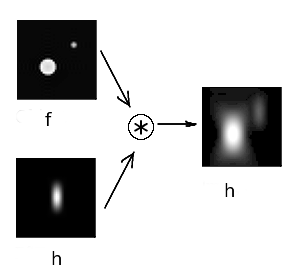
\includegraphics{conv.png}
        \caption{Приклад згортки}
        \label{fig:example-convolution}
      \end{figure}

      Саме функція спотворення й показує, по якому закону ,,збирається'' або
      розмазується пікселі зображення.
      Функція спотворення також відома як функція розподілу точки
      (англ.~PSF --- Point spread function), ядро (англ.~kernel)
      оператору спотворення, адже вона визначає, як саме кожна точка сигналу
      $f$ ,,розсіюється '' в копію PSF.
      Розмірність цієї функції, як правило, менше за розмірність самого
      зображення.

      Саме тому операція згортки також відома як суперпозіціонний
      інтеграл, а обернена операція --- розділенням сигналів.
      Але згортка є комутативною операцією --- ми можемо визначити сигнал $f$
      як PSF для сигналу $h$:
      \[ f * h = h * f \]

      Таким чином, згортка є особливою та відносно простою математичною
      операцією, а тому це досить примітно, що так багато деградацій, що
      зустрічаються повсякденно, можуть бути описаними за допомогою однієї й
      тієї ж самої операції.

      В вищенаведеному описі операції згортки було допущено, що однакова PSF
      була застосована до всіх точок сигналу $f$.
      Це припущення має місце в багатьох теоретичних викладках і має назву
      згортки з інваріантною у просторі функцією розсіювання точки.
      Але в реальних ситуаціях має місце зміна (найчастіше поступова) PSF з
      переміщенням по сигналу $f$.
      Такий випадок називається згорткою зі змінною у просторі PSF.
      В таких ситуаціях треба використовувати інші алгоритми деконволюції для
      відновлення зображення.\cite{book2}

      Розглянемо типові функції спотворення:
      \begin{figure}
        \centering
        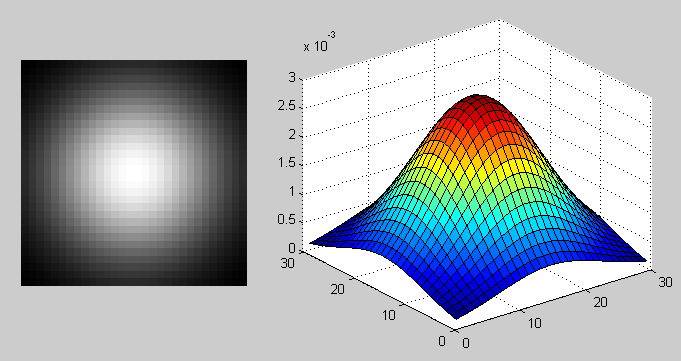
\includegraphics[width=\linewidth]{gaussian-blur.png}
        \caption{PSF у випадку розмиття за Гаусом}
        \label{fig:gaussian-blur}
      \end{figure}
      \begin{figure}
        \centering
        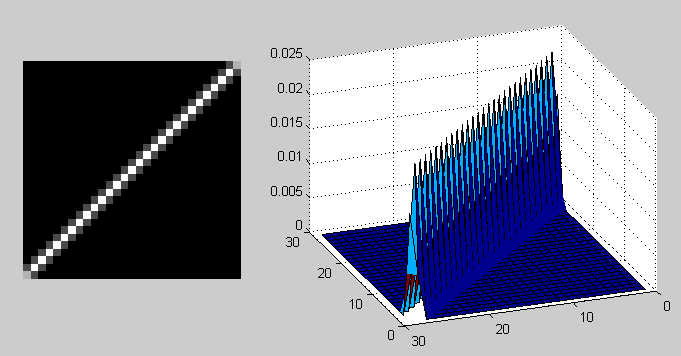
\includegraphics[width=\linewidth]{motion-blur.png}
        \caption{PSF у випадку змазу}
        \label{fig:motion-blur}
      \end{figure}
      \clearpage
    \subsection{Модель шуму}
      Доданок $n$ у формулі~\eqref{eq:model} відповідає за шум.
      Причини шуму в цифрових сенсорах можуть бути самими різними, але основні
      --- це теплові коливання.

      На величину шуму також впливає ряд факторів, а саме: значення ISO, тип
      матриці, розмір пікселя, температура, електромагнітні наведення тощо.
      У більшості випадків шум розподілений за законом Гауса(який задається
      двома параметрами --- математичним очікуванням і дисперсією):
      \begin{equation}
        f\left( x; \mu; \sigma \right) = \frac{1}{\sigma \sqrt{2 \pi}}
        e^{-\frac{\left( x - \mu \right)^2}{2 \sigma^2}}
        \label{eq:gaussian-blur}
      \end{equation}

      Такий шум характеризується рівномірною спектральною щільністю, нормально
      розподіленим значенням амплітуди та адитивним способом впливу на сигнал.

      Термін ,,адитивний'' означає, що даний шум підсумовується з
      корисним сигналом.

      Також важливим припущенням щодо шуму є те, що він не корелює з
      зображенням й не залежить від координат пікселю.
      \clearpage
    \subsection{Обернена згортка як метод відновлення}
      Процеси, спрямовані на те, щоби усунути деградації з сигналів (не лише
      тих, що обумовлені згорткою) називають процесами відновлення.
      Одним з таких процесів є деконволюція.

      Деконволюція, або обернена згортка --- операція, що є
      оберненою до згортки двох сигналів.
      Можливість ,,пере"=фокусувати'' розмите зображення після того, як воно
      було зняте (використовуючи певні обрахунки) може бути надзвичайно
      корисним, наприклад, коли неможливо зняти заново фотографію.

      Деконволюція має за собою мету обернути деградації сигналів, що були
      отримані через операцію згортки.
      Існують й інші види деградацій, але обернена згортка, зазвичай, не в
      змозі допомогти із ними.

      Під час роботи з цифровим зображенням ми говоримо про відновленні
      зображення, або, більш конкретніше, об деконволюції зображення.
      Оскільки цей процес намагається отримати сигнал до того, як він зазнав
      певної деградації, маючи лише цей деградований сигнал, деконволюція може
      бути класифікована як зворотна задача, а отже й математика
      зворотних задач тісно пов’язана з розумінням та розробкою алгоритмів
      деконволюції.

      \begin{figure}
          \minipage{0.32\textwidth}
            
\includegraphics[width=\linewidth]{Aorig.png}
            \caption{Початкове зображення}\label{fig:orig-img}
          \endminipage\hfill
          \minipage{0.32\textwidth}
            
\includegraphics[width=\linewidth]{AOrig.jpg}
            \caption{Розмите зображення}\label{fig:conv-img}
          \endminipage\hfill
          \minipage{0.32\textwidth}
            
\includegraphics[width=\linewidth]{ADecon.jpg}
            \caption{Відновлене зображення}\label{fig:deconv-img}
          \endminipage\hfill
      \end{figure}

      Приклад роботи деконволюції зображення наведений на
      Рис.~\ref{fig:orig-img}--\ref{fig:deconv-img}.
      Як видно з цієї ілюстрації, процес оберненої згортки відновив багато
      деталей, що були ,,втрачені'' під час розмиття.
      Також треба звернути увагу на те, що відновлене зображення має певні
      цяточки, які були відсутні на початковому зображенні.
      Ці цяточки є прикладом артефактів (небажаним ,,побічним ефектом'')
      деконволюції.\cite{deconvolve-index}
      \paragraph{Взаємозамінність згортки та деконволюції}
        Операція згортки не завжди пов’язана з деградацією сигналу.
        Насправді, за допомогою ,,правильної'' PSF, згортка може прибрати розмиття
        зображення, а також проста згортка з так званим зворотним фільтром
        може фактично зробити деконволюцію попереднього перетворення.

        Таким чином, згортка та деконволюція при певних умовах можуть виконувати
        однакові дії.
      \clearpage
    \subsection{Перетворення Фур’є}
      Перетворення Фур’є --- інтегральне перетворення однієї комплекснозначної
      функції дійсної змінної на іншу.
      Тісно пов’язане з перетворенням Лапласа та аналогічне розкладу у ряд
      Фур’є для неперіодичних функцій.
      Це перетворення розкладає дану функцію на осциляторні функції.
      Перетворення Фур’є визначається за формулою~\eqref{eq:fourier-def}.
      Зворотна операція, обернене перетворення Фур’є, визначається
      формулою~\eqref{eq:invfourier-def}.
      \begin{equation}
        F\left( \omega \right) = \int_{-\infty}^\infty f\left( t \right) e^{-i
        \omega t }\,dt
        \label{eq:fourier-def}
      \end{equation}
      \begin{equation}
        f\left( t \right) = \frac{1}{2 \pi} \int_{-\infty}^\infty F\left(
        \omega \right) e^{i \omega t}\, d\omega
        \label{eq:invfourier-def}
      \end{equation}

      Одна з властивостей перетворення Фур’є --- перетворення Фур’є від
      згортки.
      Ящко $f\left( x \right)$, $g\left( x \right)$ та $h\left( x \right)$ ---
      інтегровані функції, а $F\left( \omega \right)$, $G\left( \omega
      \right)$
      та $H\left( \omega \right)$ --- їх відповідні перетворення Фур’є, то має
      місце наступне:
      \begin{quote}
        Якщо $h\left( x \right) = \left( f \ast g \right)\left( x \right)$,
        тоді $H\left( \omega \right) = F\left( \omega \right) G\left( \omega
        \right)$
      \end{quote}
      \paragraph{Наслідок з теореми про згортку}
        З рівняння~\eqref{eq:convolution-2d} видно, що для знаходження $f$ з $g$
        потрібно розв’язати велику систему рівнянь.
        Але, якщо скористатися теоремою про згортку та перетворення Фур’є,
        можна перейти від нетривіальної операції згортки в просторі до
        звичайного по елементному множенню у частнотній області.
        А саме, процес спотворення можна переписати наступним чином:
        \begin{equation}
          G\left( u, v \right) = H\left( u, v \right) F\left( u, v \right) +
          N\left( u, v \right)
          \label{eq:deffect-fourier}
        \end{equation}
      \clearpage
  \section{Алгоритми деконволюції}
    \subsection{Види деконволюції}
      Деконволюцію можна класифікувати за інформацією, що відома про функцію
      розсіювання точки:
      \begin{itemize}
        \item Несліпа.
          У цьому випадку PSF відома заздалегідь.
        \item Сліпа.
          У цьому випадку функція розсіювання точки не відома заздалегідь, а
          тому потрібно використовувати інші методи відновлення зображення.
          Ця задача є набагато складнішою за несліпу деконволюцію, адже
          необхідно знайти оригінал зображення лише за деградованим зображенням.
          Для того, щоб рішення цієї задачі було можливим необхідно вказати
          певні межі можливого розв’язку.
          Насправді, вказувати межі може бути необхідно й при вирішенні задачі
          несліпої деконволюції, адже часто існує багато різних розв’язків.
        \item Випадки, коли відома частина PSF.
      \end{itemize}
      \clearpage
    \subsection{Інверсна фільтрація}
      Одним з найочевидніших рішень є ділення всього
      рівняння~\eqref{eq:deffect-fourier} на $H\left( u, v \right)$, в
      результаті чого ми отримаємо наближення до початкового зображення
      $\hat{F}\left( u, v \right)$:

      \begin{equation}
        \hat{F}\left( u, v \right) = F\left( u, v \right) + \frac{N\left( u, v
        \right)}{H\left( u, v \right)}
        \label{eq:inverse-filter}
      \end{equation}

      Це рівняння описує процес, що має назву інверсна фільтрація.
      Проте, на практиці він майже ніколи на приводить до гарного результату.
      Для того, щоб зрозуміти, чому так трапляється, достатньо подивитися на
      останній доданок з рівняння~\eqref{eq:inverse-filter} --- якщо функція $H\left(
      u, v \right)$ приймає значення, близькі до нульових, то цей доданок буде
      домінуючим.
      Саме так і трапляється на практиці.
      % ~\cite{hons}

      Для ілюстрації цього ефекту, візьмемо початкове зображення, перетворимо
      його у напівтонове й отримаємо його спектр.
      \begin{figure}[!htb]
        \minipage{0.32\textwidth}
          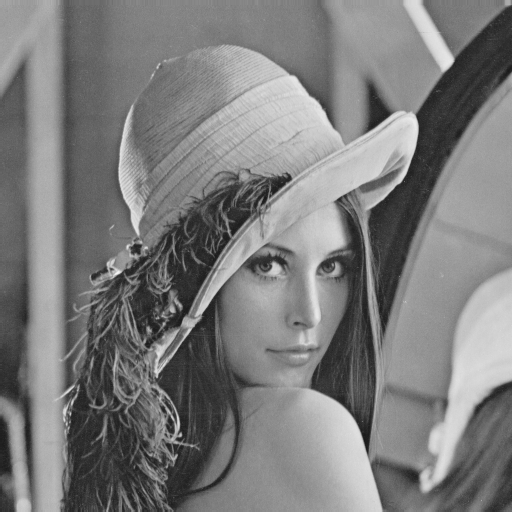
\includegraphics[width=\linewidth]{Lenna-gray.png}
          \caption{Початкове зображення}\label{fig:Lenna-gray-img}
        \endminipage\hfill
        \minipage{0.32\textwidth}
          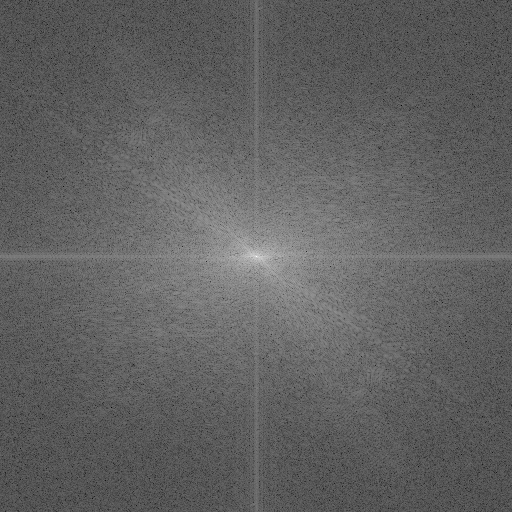
\includegraphics[width=\linewidth]{Lenna-ampl.png}
          \caption{Амлітудний спектр}\label{fig:Lenna-ampl-img}
        \endminipage\hfill
        \minipage{0.32\textwidth}
          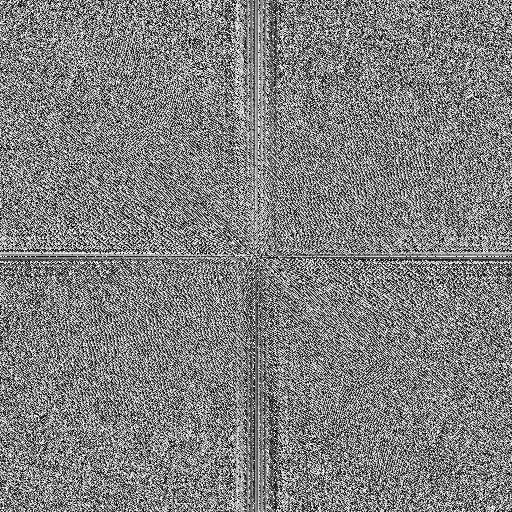
\includegraphics[width=\linewidth]{Lenna-phase.png}
          \caption{Фазовий спектр}\label{fig:Lenna-phase-img}
        \endminipage\hfill
      \end{figure}

      Як видно з амплітудного спектру, зображеному на
      Рис.~\ref{fig:Lenna-ampl-img}, його значення змінюється дуже швидко ---
      на декілька порядків.
      В центрі --- максимальне значення (порядку $10^6$) та швидко зменшується
      до нульових по краях.
      Саме через це інверсна фільтрація буде працювати лише при нульових або
      близько нульових значеннях шуму.
      Результат можна побачити на
      Рис.~\ref{fig:Lenna-img}--\ref{fig:Lenna-b1e-8deconv}.

      \begin{figure}[htb]
        \minipage{0.32\textwidth}
          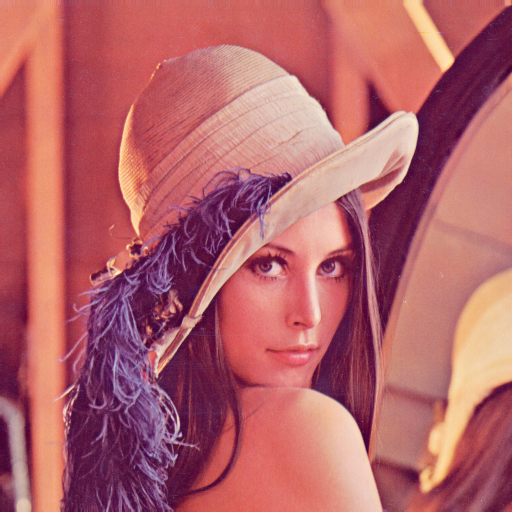
\includegraphics[width=\linewidth]{Lenna.png}
          \caption{Початкове зображення}\label{fig:Lenna-img}
        \endminipage\hfill
        \minipage{0.32\textwidth}
          
\includegraphics[width=\linewidth]{Lenna-blurred.png}
          \caption{Розмите зображення}\label{fig:Lenna-blurred-img}
        \endminipage\hfill
        \minipage{0.32\textwidth}
          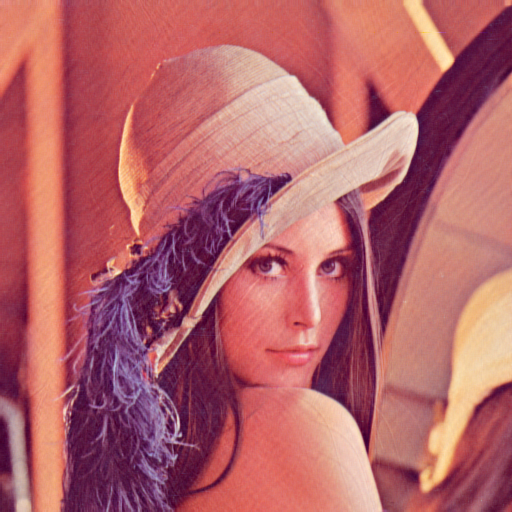
\includegraphics[width=\linewidth]{Lenna-b0deconv.png}
          \caption{Відновлене зображення}\label{fig:Lenna-b0deconv}
        \endminipage\hfill

        \minipage{0.32\textwidth}
          
\includegraphics[width=\linewidth]{Lenna-b1e-9.png}
          \caption{Зображення з шумом $10^{-9}$}\label{fig:Lenna-b1e-9}
        \endminipage\hfill
        \minipage{0.32\textwidth}
          
\includegraphics[width=\linewidth]{Lenna-b5e-9.png}
          \caption{Зображення з шумом $5\cdot10^{-9}$}\label{fig:Lenna-b5e-9}
        \endminipage\hfill
        \minipage{0.32\textwidth}
          
\includegraphics[width=\linewidth]{Lenna-b1e-8.png}
          \caption{Зображення з шумом $10^{-8}$}\label{fig:Lenna-b1e-8}
        \endminipage\hfill

        \minipage{0.32\textwidth}
          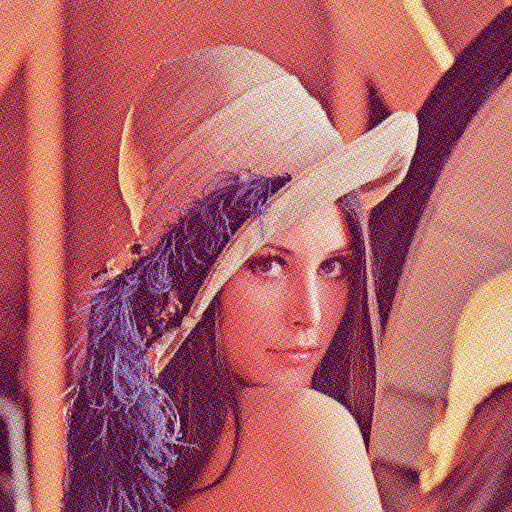
\includegraphics[width=\linewidth]{Lenna-b1e-9deconv.png}
          \caption{Відновлене зображення з шумом $10^{-9}$}\label{fig:Lenna-b1e-9deconv}
        \endminipage\hfill
        \minipage{0.32\textwidth}
          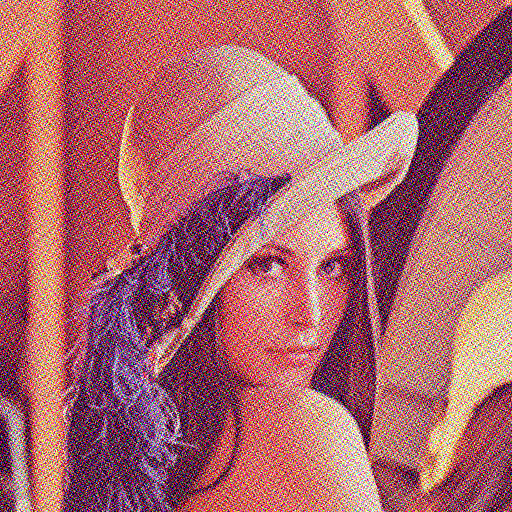
\includegraphics[width=\linewidth]{Lenna-b5e-9deconv.png}
          \caption{Відновлене зображення з шумом $5\cdot10^{-9}$}\label{fig:Lenna-b5e-9deconv}
        \endminipage\hfill
        \minipage{0.32\textwidth}
          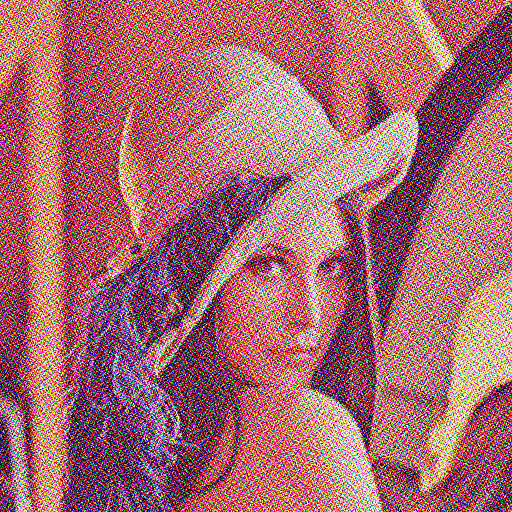
\includegraphics[width=\linewidth]{Lenna-b1e-8deconv.png}
          \caption{Відновлене зображення з шумом $10^{-8}$}\label{fig:Lenna-b1e-8deconv}
        \endminipage\hfill
      \end{figure}
      Гарно видно, що додавання навіть дуже незначного шуму призводить до
      значних помилок, що сильно обмежує корисність методу.
      \clearpage
    \subsection{Фільтр Вінера}
      Існують методи, що враховують існування шуму на зображенні.
      Один з самих відомих й старіших --- фільтр Вінера (Wiener).

      В математичній моделі алгоритму Вінера як зображення, так і шум
      розглядаються як випадкові (стохастичні) процеси.
      Основна ідея --- знайти таку оцінку $f^\prime$ неспотвореного
      (початкового) зображення $f$, таку, щоб середньоквадратичне відхилення
      цих величин було мінімальним.

      Вінер знайшов, що мінімум цього відхилення досягається на функції в
      частотній області:
      \begin{equation}
        \hat{F}\left( u, v \right) = \left( \frac{1}{H\left( u, v \right)}
        \frac{\left| H\left( u, v \right)\right|}{\left|H\left( u, v
          \right)\right|^2 + \frac{S_\eta\left( u, v \right)}{S_f\left( u, v
          \right)}} \right) G\left( u, v \right)
        \label{eq:wiener1}
      \end{equation}

      Функцією $S$ тут позначені енергетичні спектри шуму та початкового
      зображення.
      Оскільки ці величини майже ніколи не відомі, то дробь
      $\frac{S_\eta}{S_f}$ замінюють на деяку константу $K$, яку можна
      охарактеризувати як співвідношення сигналу до шуму.

      Всі дії в алгоритмі Вінера виконуються в частнотній області, а тому
      потрібно застосувати перетворення Фур’є до початкових даних, я
      застосувати обернене перетворення Фур’є до результату.
      \clearpage
    \subsection{Фільтрація за Тихоновим}
      Наступний метод --- згладжуюча фільтрація методом найменших
      квадратів зі зв’язком, або фільтрація за Тихоновим,
      Тихоновська регуляризація.
      Його ідея полягає в формулюванні завдання в матричному вигляді й
      подальшому рішенні отриманої задачі оптимізації.

      Це рішення записується у вигляді:
      \begin{equation}
        \hat{F}\left( u, v \right) = \left( \frac{H^\ast\left( u, v
        \right)}{\left|H\left( u, v \right)\right|^2 + y\left|P\left( u, v
        \right)\right|^2} \right) G\left( u, v \right)
        \label{eq:tihonov1}
      \end{equation}

      У рівнянні~\eqref{eq:tihonov1} $y$ --- параметр регуляризації, а
      $P\left( u, v \right)$ --- перетворення Фур’є оператору Лапласу (матриця
      $3\times3$).
      \clearpage
    \subsection{Метод Люсі"=Річардсона}
      Ще одне досить цікаве рішення було незалежно знайдене Річардсоном у
      1972~році та Люсі у 1974~році.
      Його головною особливістю є те, що він не є лінійним, на відміну від
      попередніх.
      Через це він, потенціально, може дати кращий результат.
      Друга особливість --- цей метод є ітеративним, через це існують деякі
      складності, що пов’язані з критерієм зупинки ітерацій.

      Основна ідея полягає в використанні методу максимальної
      правдоподібності, для чого припускається, що спотворююча функція
      описується певним розподілом Пуасону.

      Також, на відміну від попередніх методів, перетворення Фур’є не
      використовується в цьому методі:
      \begin{equation}
        \hat{f}_{k+1}\left( x, y \right) = \hat{f}_k \left( x, y \right)\left(
        h\left( -x, -y \right) \ast \frac{g\left( x, y \right)}{h\left( x, y
          \right) \ast \hat{f}_k\left( x, y \right)} \right)
        \label{eq:lr1}
      \end{equation}

      Цей метод набув широкого застосування для обробки астрономічних
      фотознімків --- у цей сфері використання деконволюції, як методі
      відновлення зображення, є стандартом де-факто.
      Обчислювальна складність методу досить велика --- обробка середньої
      фотографії, в залежності від кількості ітерацій, може займати години й
      навіть дні.

      Алгоритм можна записати у трохи іншому, більш легкому для реалізації,
      вигляді.
      Точки розмитого зображення можуть бути представленими у формі суми:
      \[ d_i = \sum_j p_{ij} u_j, \]
      де $p_{ij}$ --- частина інтенсивності, що розсіялася з позиції $j$ в
      позицію $i$, $u_j$ --- $j$-та точка зображення, $d_i$ --- $i$-та точка
      отриманого розмитого зображення.\cite{richardson-hadley}

      Головна ідея полягає в тому, що необхідно підрахувати найбільш"=вірогідне
      значення $u_j$, якщо відомі $d_i$ та $p_{ij}$.

      \begin{equation}
        u_j^{(t+1)} = u_j^{(t)} \sum_i \frac{d_i}{c_i} p_{ij}
        \label{eq:rl-deconv}
      \end{equation}

      \[c_i = \sum_j p_{ij} u_j^{(t)}\]
      \clearpage
    \subsection{Методи сліпої деконволюції}
      Зараз набуває популярності сімейство методів, об’єднані під загальною
      назвою сліпа деконволюція (blind deconvolution).
      В попередніх методах вважалося, що функція спотворення PSF відома.
      Але в реальності найчастіше PSF відома лише приблизно за характером
      спотворення.
      Сліпа деконволюція як раз має за собою мету врахувати цей факт.
      Принцип у багатьох випадках досить простий --- знаходиться деяке
      наближення PSF, за одним із методів робиться деконволюція, після чого за
      деяким критерієм оцінюється ступінь якості відновленого зображення й
      уточнюється PSF для подальшої ітерації.
      \clearpage
\chapter{МАТЕМАТИЧНЕ МОДЕЛЮВАННЯ}
  У процесі спотворення з кожного пікселя вихідного зображення виходить деяке
  пляма у разі розфокусуванні і відрізок для випадку звичайного змазу.
  Все це один на одного накладається і в результаті ми отримуємо спотворене
  зображення ---- це називається згорткою, або конволюцієй, зображення.
  Те, за яким законом розмазується один піксель і називається функцією
  спотворення.
  Інші синоніми --- PSF (Point spread function, тобто функція розподілу
  точки), ядро оператора спотворення, kernel та інші.

  Щоб відновити вихідне зображення нам необхідно якимось чином обернути процес
  згортки, при цьому не забуваючи про шум.
  Але це не така проста задача --- якщо діяти, що називається, ,,напряму'', то
  вийде величезна система рівнянь, яку вирішити за прийнятний час неможливо.

  Але на допомогу до нас приходить перетворення Фур'є і теорема про згортку,
  яка свідчить, що операція згортки в просторовій області еквівалентна
  звичайному множенню в частотній області (причому множення по елементне, а не
  матричне.
  Відповідно, операція зворотна згортку еквівалентна діленню в частотній
  області.

  Будемо розглядати процес деконволюції на прикладі фільтру Вінера (більшість
  інших методів дають майже ті ж самі результати).

  Основна задача --- отримати оцінку функції розподілу точки.
  \clearpage
  \section{Методи наближення функції розподілу точки}
    \subsection{Моделювання}
      Моделювання PSF є дуже непростою й трудомісткою проблемою.

      Сучасні об’єктиви складаються з десятків різних оптичних лінз та оптичних
      елементів, частина з яких мають асферичну форму.
      Також, кожен сорт скла, з якого виготовляються лінзи, має свої унікальні
      характеристики заломлення променів із тією чи іншою довжиною хвилі.

      Отже, задача моделювання PSF в такій складній оптичній системі, з
      урахуванням впливу діафрагм, перевідбиттів тощо стає практично неможливою
      задачею.

      Рішення цієї задачі доступно лише, можливо, розробникам сучасних
      об’єктивів.
      \clearpage
    \subsection{Безпосереднє спостереження}
      Ідея цього методу полягає в безпосередньому спостереженні перетворення
      точки під час спотворення.

      Оскільки PSF показує, на що перетворюється кожна точка початкового
      зображення, можливо отримати шукану PSF отримавши зображення білої точки
      на чорному фоні після спотворення.

      Хоча цей метод здається простим, існує багато нюансів.
      Наприклад, PSF може бути різною для хвиль різної довжини.
      PSF може залежати від координат пікселю.

      Також потрібно пам’ятати, що знайдена таким чином PSF буде правдивою
      лише при тому ж самому спотворенні, що в багатьох випадках складно
      отримати.

      Якщо просто розпечатати на чорному фоні білу точку, то цього буде
      недостатньо.
      Потрібно більше контрасту між точкою й фоном.
      Для цього можна, наприклад, зробити в чорному фоні точкову діру, та
      світити скрізь неї джерелом світла.
      \clearpage
    \subsection{Обчислення або непряме спостереження}
      Цей метод напряму залежить від можливості отримати неспотворене
      зображення, а отже має дуже малу область застосування.

      З формули~\eqref{eq:deffect-fourier} можна отримати образ перетворення
      Фур’є від функції розподілу точки $H\left( u, v \right)$ як результат
      ділення образу Фур’є спотвореного зображення $G\left( u, v \right)$ на
      Фур’є перетворення від початкового зображення $F\left( u, v \right)$.

      Цей метод показує, що ми можемо розглядати початкове зображення $f\left(
      x, y \right)$ як функції спотворення для $h\left( x, y \right)$

      Для найкращого ефекту необхідно поставити фотоапарат на штатив й
      сфотографувати певний об’єкт, після чого зробити розмитий знімок того ж
      самого об’єкту з тієї ж самої позиції.
      \clearpage
  \section{Боке}
    Розглянемо трохи теорії розфокусування стосовно реальної оптики.

    Ідеальний об’єктив має PSF у вигляді кола, відповідно кожна точка
    перетворюється в коло деякого діаметру.
    До речі, саме через це з першого погляду здається, що дефокус просто
    розтушовує все зображення.
    Це ж пояснює і те, чому розмиття за Гаусом, здійснене у фоторедакторах
    зовсім не схоже на той малюнок фону (його ще називають боке), який
    ми бачимо у об’єктивів.
    Насправді це два різних типи розмиття --- за Гаусом кожна точка
    перетворюється на нечітка пляма (дзвін Гауса), а дефокус кожну точку
    перетворює в коло.
    Відповідно і різні результати.

    Але ідеальних об’єктивів не існує, і в реальності ми отримуємо те чи інше
    відхилення від ідеального кола.
    Саме це і формує неповторний малюнок боке кожного об’єктива.

    Боке можна умовно розділити на три типи:
    \begin{itemize}
      \item Нейтральне. Це максимальне наближення до кола.
      \item М’яке. Коли краю мають меншу яскравість, ніж центр
      \item Жорстке. Коли краю мають велику яскравість, ніж центр.
    \end{itemize}
    Крім того, тип боке залежить від того, чи передній це фокус, чи
    задній.
    Тобто, чи фотоапарат сфокусований перед об’єктивом чи за ним.
    Тільки нейтральне боке не залежить від фокусу.

    \begin{figure}[h]
      \minipage{0.32\textwidth}
        \centering
        
\includegraphics{neutral_boke.png}
        \caption{Нейтральне боке}
        \label{fig:neutral_boke}
      \endminipage\hfill
      \minipage{0.32\textwidth}
        \centering
        
\includegraphics{soft_boke.png}
        \caption{М’яке боке}
        \label{fig:soft_boke}
      \endminipage\hfill
      \minipage{0.32\textwidth}
        \centering
        
\includegraphics{hard_boke.png}
        \caption{Жорстке боке}
        \label{fig:hard_boke}
      \endminipage\hfill
    \end{figure}
    \clearpage
  \section{Крайові ефекти}
    Описані методи можна й потрібно використовувати для побудови PSF при
    відновленні спотворених зображень.
    Оскільки від того, як добре ця функція наближена до реальної, залежить
    кість відновленого зображення.

    Якщо передбачувана та реальні PSF розбігаються, то будуть спостерігатися
    численні артефакти у вигляді ,,дзвону'', ореолів і зниження чіткості.
    У більшості випадків передбачається форма PSF у вигляді кола, проте для
    досягнення максимального ступеня відновлення рекомендується
    експериментувати з формою цієї функції, спробувавши кілька варіантів від
    поширених об’єктивів.

    Якщо безпосередньо застосувати фільтр Вінера, то на краях зображення буде
    своєрідний ,,дзвін''.
    Його причина полягає в наступному --- коли робиться деконволюція для тих
    точок, які розташовані на краях, то при складанні не вистачає даних з
    пікселів, які перебувають за краями зображення і вони приймаються або
    рівним нулю, або беруться з протилежного боку (залежить від реалізації
    фільтра Вінера і перетворення Фур’є). Виглядає це так:
    \begin{figure}[h]
      \centering
      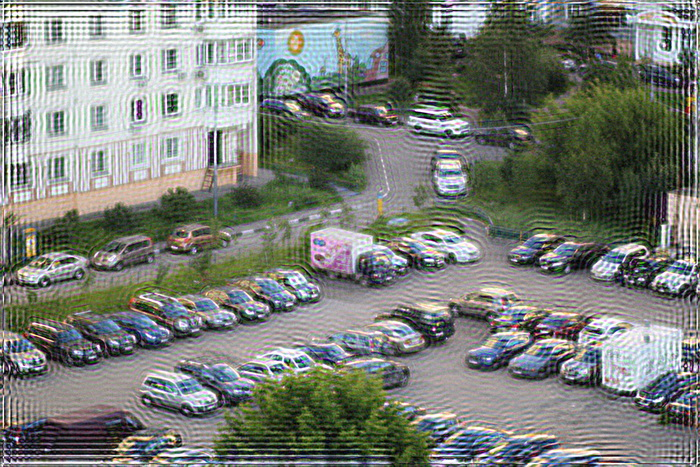
\includegraphics[width=\linewidth]{edge-artifact.jpg}
      \caption{Артефакт ,,дзвону''}
      \label{fig:edge-artifact}
    \end{figure}

    Одно з рішень полягає в попередній обробці країв зображення.
    Вони розмиваються за допомогою тієї ж самої функції розподілу точки.
    На практиці це реалізується наступним чином --- береться вхідне,
    спотворене, зображення $F\left( x, y \right)$, розмивається за допомогою
    PSF, тим самим отримуємо $F^\prime\left( x, y \right)$.
    Після цього отримуємо остаточне вхідне зображення як суму $F\left( x, y
    \right)$ та $F^\prime\left( x, y \right)$ з використанням вагової функції,
    яка по краях зображення приймає значення $1$, а всередині зображення,
    на відстані більше чи рівної радіусу PSF від країв зображення, приймає
    значення $0$.
    Результат отримуємо наступний (вже без ,,дзвону'' по краях):
    \begin{figure}[h]
      \centering
      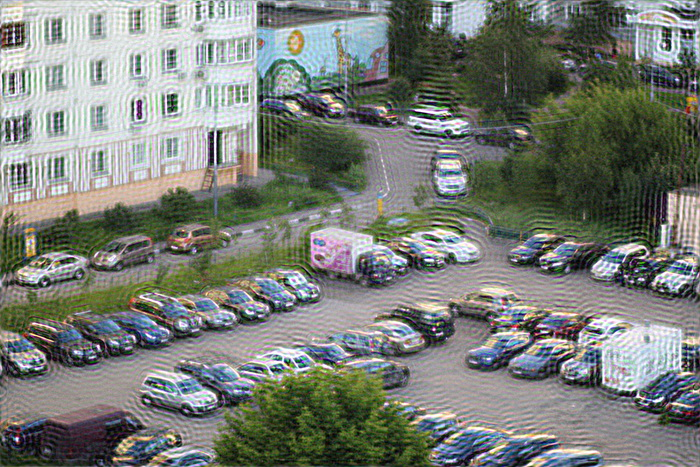
\includegraphics[width=\linewidth]{edge-fixed.jpg}
      \caption{Зображення без артефакту ,,дзвону''}
      \label{fig:edge-fixed}
    \end{figure}

\chapter{ПРОГРАМНА РЕАЛІЗАЦІЯ}
  Було розроблено пакет прикладних програм, що демонструють відновлення
  змазаних і розфокусованих зображень.

  Були використані наступні технологічні рішення:
  \begin{itemize}
    \item мова програмування C++;
    \item набір бібліотек Qt4;
    \item бібліотека FFTW, як найшвидша реалізація перетворення Фур’є, що
      розповсюджується під ліцензією GPLv3.
  \end{itemize}

  \begin{figure}[h]
    \centering
    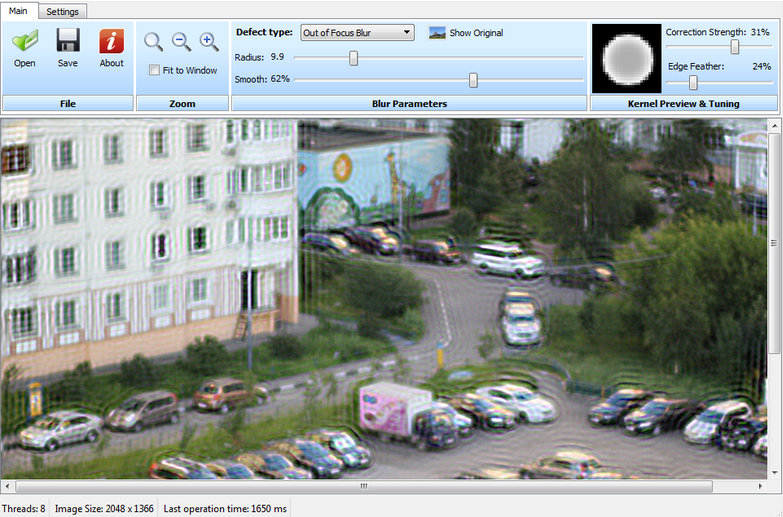
\includegraphics[width=\linewidth]{gui.png}
    \caption{Знімок екранної форми}
    \label{fig:gui}
  \end{figure}

  Основні можливості розробленого програмного засобу:
  \begin{itemize}
    \item Швидкодія.
      Обробка зображення розміром $2048\times1500$ пікселів займає близько
      $300$~мс в режимі Preview (коли можливо корегувати PSF) й $1500$~мс у
      фінальному режимі.
    \item Можливість вибору параметрів у Realtime режимі.
      Немає необхідності натискати кнопку Preview, усе робиться автоматично.
    \item Уся обробка проводиться над зображенням у повному розмірі.
    \item Можливість корегування PSF.
  \end{itemize}
\chapter{ОХОРОНА ПРАЦІ}
  За сучасних умов, комп’ютери набули широкого поширення.
  Вони застосовується на кожному підприємстві для організації діяльності
  праці.
  Комп’ютери є невід’ємним і, найчастіше, одним із головних інструментів при
  виконанні поставлених завдань.

  Даних розділ дипломної роботи носить рекомендаційний характер та має
  відношення до робіт одного типу, а отже подальші рекомендації будуть
  пов’язані зі специфікою роботи з персональними комп’ютерами.

  Основним нормативним документом щодо забезпечення охорони праці користувачів
  персонального комп’ютера є НПАОП~0.00-1.28-10\cite{npaop128} та
  ДНАОП~0.00-1.31-99\cite{dnaop131}.
  \clearpage
  \section{Характеристика робочого місця}
    Робоче приміщення знаходиться на четвертому поверсі в цегляному будинку.
    Найближчі будівлі знаходяться на значній відстані та не впливають на
    рівень проникнення світла.
    План приміщення зображений на рис.~\ref{fig:plan}.
    \begin{figure}[ht]
      \centering
      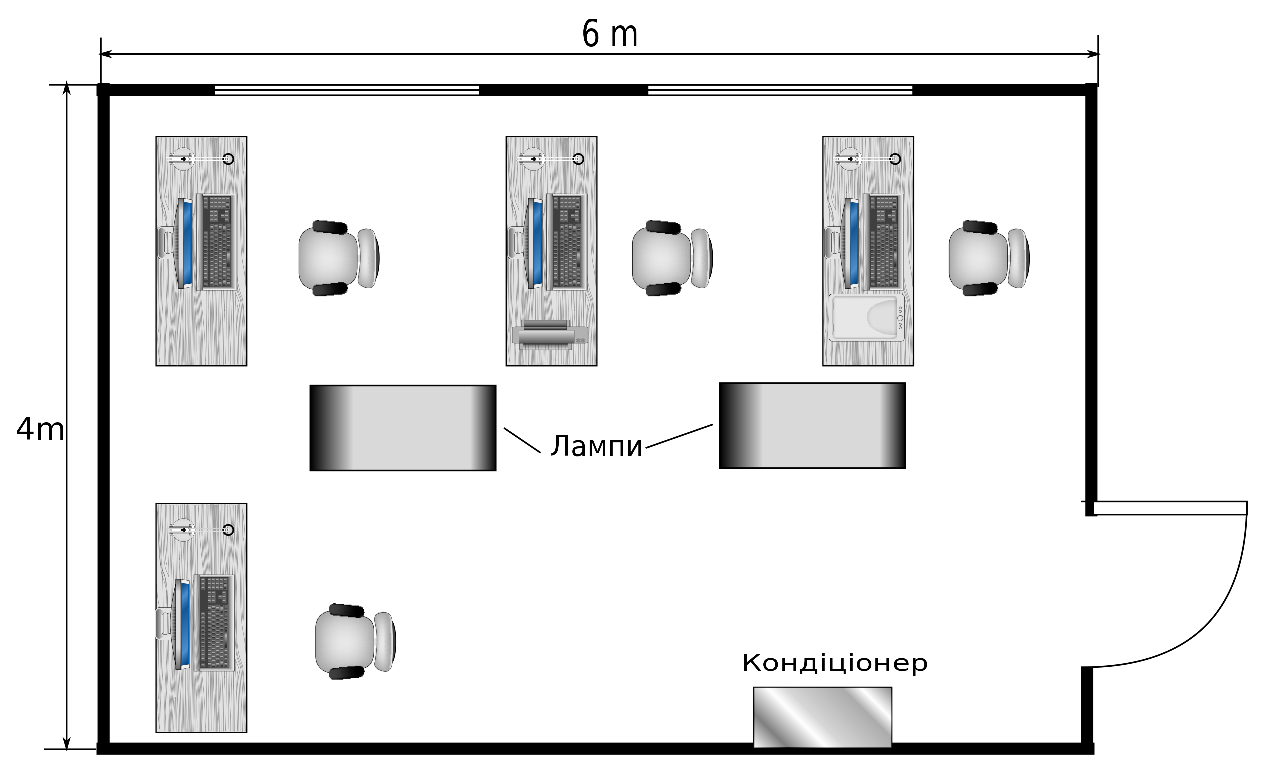
\includegraphics[width=\linewidth]{plan2.eps}
      \caption{План приміщення}
      \label{fig:plan}
    \end{figure}

    Санітарно"=гігієнічні вимоги щодо влаштування приміщень, в яких працівники
    працюють на персональних комп’ютерах, параметрів виробничого середовища,
    організації та обладнання робочих місць, режимів праці та відпочинку при
    роботі з відеотерміналами (ВДТ) і профілактичних медоглядів наведено
    у~\cite{npaop128}.

    Згідно з санітарними нормами з цього документу розмір площі для одного
    робочого місця оператора персонального комп’ютера повинен бути не менше
    $6.0$~м$^2$, а об’єм --- не менше $20.0$~м$^3$.
    Довжина кімнати --- $6.0$~м, ширина --- $4.0$~м, висота ---
    $2.7$~м.
    Маються також два вікна ($2.0$~м~$\times$~$1.6$~м), які спрямовані
    на північ.
    Отже, площа приміщення складає
      \[
        S = 6 \times 4 = 24~\text{м}^2,
      \]
    а обсяг
      \[
        V = 24 \times 2.7 = 64.8~\text{м}^2.
      \]
    Кожне робоче місце обладнане електронно"=обчислювальними машинами з
    РК"=моніторами Samsung LN32D403E2DXZA.
    У приміщенні постійно працює до чотирьох чоловік.
    Отже, на кожне робоче місце припадає по $6.0$~м$^2$ площі в об’ємі не
    менше, ніж $20.0$~м$^3$, що відповідає санітарним нормам.

    Санітарні норми також передбачають, що при розміщенні робочих столів з
    відеотерміналами слід дотримувати такі відстані: між бічними поверхнями
    ВДТ --- $1.2$~м, відстань від тильної поверхні одного відеотерміналу до
    екрана іншого відеотерміналу --- $2.5$~м.

    Параметри столу: довжина --- $1450$~мм, ширина --- $740$~мм, висота ---
    $730$~мм.
    Відстань між робочими столами також відповідає санітарним нормам, а саме
    не є меншою, ніж $2.0$~м.

    Робочі стільці є підйомно"=поворотні, регульовані за висотою, кутом нахилу
    сидіння та спинки.
    Поверхня сидіння --- плоска, а передній край --- заокруглений.
    Регулювання за кожним із параметрів здійснюється незалежно, легко та
    надійно фіксується.

    Екран ВДТ розташовується на відстані $670$~мм до очей користувача, що
    є оптимальною відстанню.
    Саме розташування екрану ВДТ забезпечує зручність зорового спостереження у
    вертикальній площині під кутом $30^\circ$.

    Столи були вибрані з урахуванням наступних умов:
    \begin{itemize}
      \item поверхня столу повинна володіти властивостями, що виключають появу
        відблисків в полі зору програміста;
      \item нижня частина столу повинна бути сконструйована так, щоб працівник
        міг зручно сидіти, не був вимушений підтискати ноги;
      \item висота столу повинна бути вибрана з урахуванням можливості сидіти
        вільно, в зручній позі, при необхідності спираючись на підлокітники;
      \item конструкція столу повинна передбачати наявність висувних ящиків.
    \end{itemize}

    Робоче приміщення, що розглядається, оснащене аптечками першої медичної
    допомоги.
    \clearpage

  \section{Аналіз шкідливих і небезпечних виробничих факторів}
    \subsection{Мікроклімат}
      Висока температура повітря негативно позначається на функціональному
      стані людини.
      Оптимальні та припустимі мікрокліматичні параметри у приміщеннях повинні
      враховувати специфіку технологічного процесу при використанні ПК.
      Зокрема, технічні умови експлуатації багатьох типів комп’ютерів містять
      допустимі робочі діапазони параметрів мікроклімату:
      \begin{itemize}
        \item температура повітря має знаходитись в межах від $10$ до
          $40^\circ C$;
        \item відносна вологість має знаходитися в межах від $40$ до $90\%$.
      \end{itemize}

      За даними ВООЗ, оптимальні значення температури у приміщенні становлять
      $19$--$23^\circ C$, відносна вологість повітря --- $55\%$, швидкість
    руху повітря не повинна перевищувати на рівні обличчя $0.1$~м/с.
      При відчутному нагрівання поверхонь (більше $45^\circ C$),
      контактуючих з людиною, передбачаються засоби охолодження або ізоляції.
      Особлива увага приділяється шляхом відводу повітря, щоб виключити
      перегрівання або протяг.

      Згідно з діючими в Україні нормативними документами\cite{dsn042} для
      даної категорії робіт (легка Iа) мають місце норми, наведені у
      табл.~\ref{tab:microclimat}.

      \begin{xtable}{|c|l|c|}{3}{Параметри мікроклімату для приміщень, де
        встановлені комп’ютери}{tab:microclimat}
          \hline
            Період року & Параметр мікроклімату & Величина\\
          \hline
            \multirow{3}{*}{Холодний} & Температура повітря & $22$--$24^\circ
            C$\\
          \cline{2-3}
            & Швидкість руху повітря & до $0.1$~м/с\\
          \cline{2-3}
            & Відносна вологість & $40$--$60\%$\\
          \hline
            \multirow{3}{*}{Теплий} & Температура повітря & $23$--$25^\circ
            C$\\
          \cline{2-3}
            & Швидкість руху повітря & $0.1$~м/с\\
          \cline{2-3}
            & Відносна вологість & $40$--$60\%$\\
          \hline
      \end{xtable}

      Завдяки встановленого кондиціонера можливо індивідуальне регулювання
      роздачі повітря в приміщенні.

      В процесі роботи змінюється концентрація іонів у повітрі робочої зони.
      Нормалізуючий вплив на аероіонний склад повітря робочої зони
      забезпечують: примусова вентиляція, захисні екрани та застосування
      іонізаторів.
      Повітря, що надходить у робочі приміщення, має бути очищене від
      забруднень, в тому числі від мікроорганізмів.

      Потужність (точніше, потужність охолодження) є основною характеристикою
      будь-якого кондиціонера.
      Серед різних моделей у нашому випадку пасує модель \texttt{RAS-30 CH1}
      фірми HITACHI, яка має потужність по холоду $4.14$~кВт.
    \subsection{Шум}
      Встановлено, що шум погіршує умови праці, роблячи шкідливий вплив на
      організм людини.
      При тривалому впливі шуму на людину відбуваються небажані явища:
      знижується гострота зору, слуху, підвищується кров’яний тиск, знижується
      увага.
      Сильний тривалий шум може стати причиною функціональних змін
      серцево"=судинної і нервової систем.

      Нормативний рівень шуму не повинний перевищувати $50$~дБа\cite{dsn037}.

      У приміщенні маються внутрішні джерела постійного шуму: вентилятор
      блоків ПЕОМ($35$~дБа, $8$~годин); принтери($48$~дБа, $2$~години);
      дисковод($40$~дБа, $0.5$~години).
      Зовнішніми джерелами шуму і вібрації в приміщенні є проїжджаючі
      транспортні засоби ($40$~дБа, $8$~годин).

      Отже, в приміщенні рівень шуму є допустимим, а отже засоби захисту не
      потрібні.
    \subsection{Освітлення}
      Природне світло проникає через бічні світло"=прорізи, зорієнтовані на
      північ, і забезпечує коефіцієнт природної освітленості (КПО) не нижче
      $1.5\%$.

      Як джерело світла при штучному освітленні повинні застосовуватися, як
      правило, люмінесцентні лампи типу ЛБ.
      У даному приміщенні застосовуються лампи NORTCLIFFE HF ECO з частотою
      перетворення $46$~кГц.
      Яскравість світильників загального освітлення в зоні кутів
      випромінювання від $50^\circ$ до $90^\circ$ відносно вертикалі в
      подовжній і поперечній площинах повинна складати не більше
      $200$~кд/м$^2$, а захисний кут світильників повинен бути не більшим за
      $40^\circ$.~\cite{dbn28}

      Рівень освітленості на робочому столі в зоні розташування документів має
      бути в межах $300$--$500$~лк.
      У разі неможливості забезпечити даний рівень освітленості системою
      загального освітлення допускається застосування світильників місцевого
      освітлення, але при цьому не повинно бути відблисків на поверхні екрана
      та збільшення освітленості екрану більше ніж до $300$~лк.

      Розраховуємо загальний світловий потік для освітлення площі робочого
      приміщення:
      \begin{equation}
        F_{n} = \frac{E_n S K_\text{зап} Z}{\eta},
        \label{eq:f-n}
      \end{equation}
      де $E_n$ --- нормоване значення штучної освітленості, $S$ --- площа
      приміщення, $K_\text{зап}$ --- коефіцієнт запасу, $Z$ --- коефіцієнт
      нерівномірності освітлення, $\eta$ --- коефіцієнт використання
      світильника.
      \[ F_{n} = (0.8 \times 24 \times 2 \times 1.5) / 0.55 = 1.2~\text{лм} \]

      Необхідна кількість світильників визначається за формулою:
      \begin{equation}
        n = \frac{F_n}{F_1},
        \label{eq:n}
      \end{equation}
      де, $F_n$ --- потрібний загальний світовий потік, $F_1$ --- світловий
      потік, створюваний одним світильником.
      \[ n = 1.2 / 0.5 = 2~\text{шт} \]
    \subsection{Електробезпека}
      Згідно з Правилами улаштування електроустановок (ПУЕ, 2009~р.) дане
      приміщення відноситься до категорії приміщень без підвищеної безпеки.

      Електроживлення однофазне $220$~В з глухо"=заземленою нейтраллю,
      виконане 3-х провідних проводом.
      Для підключення обладнання встановлені розетки з заземлюючим контактом.
      Провідники заземлення приєднані до загального контуру заземлення.
      Опір загального становить $3$~Ом.
      Заземлення корпусів ЕОМ та іншого обладнання здійснюється через вилку
      підключення о джерела живлення.

      Дане робоче приміщення відповідає вимогам~\cite{dnaop131}.
    \subsection{Пожежна безпека}
      Дане приміщення відноситься до категорії B, класу П-IIа.
      До цієї зони відносяться приміщення, у яких використовуються тверді чи
      волокнисті речовини, нездатні переходити в зважений стан\cite{napb}.
      У приміщенні є пальні речовини: волокнисті(папір), тверді(дерево),
      пластмаси.

      Тому що ПЕОМ мають велику вартість, з огляду на категорію пожежної
      небезпеки приміщення, будинку з використанням ПЕОМ повинні бути I і II
      ступеня вогнестійкості (тобто всі конструктивні елементи повинні бути
      неспаленими).
      Фактично приміщення відповідає цим нормам (основні будівельні матеріали
      --- цегла, бетон, скло).

      У коридорах будинку установлюються пожежні крани.
      Вода використовується для гасіння пожеж у допоміжних службово"=побутових
      приміщеннях.
      Пожежні крани розташовують на висоті $1.35$~м від підлоги в найбільш
      доступних місцях.

      Для гасіння пожежі в початковій стадії його виникнення в приміщенні
      встановлено 2 вогнегасника: ВВ-5(з) (вогнегасник вуглекислотний закачний
      ємністю $1.3$~л.

      Для запобігання пожежі в приміщенні прийняті такі міри:
      \begin{itemize}
        \item передбачено вільний доступ до мережних рубильників і вимикачів;
        \item інструктаж з пожежної безпеки і періодичний контроль знань про
          правила пожежної безпеки;
        \item встановлені два димових сповіщувача ИПД-1;
        \item заборона використання електронагрівальних приладів;
        \item маються 2 вогнегасник ВВ-5(з);
        \item двері на шляху проходження людей відкриваються назовні;
        \item ширина загального коридору, ширина дверей, висота дверей
          відповідають нормативним значенням ОНТП 24-86;
        \item призначено відповідального за пожежну безпеку в приміщенні.
      \end{itemize}
      \clearpage
  \section{Інструкція з техніки безпеки}
    Дії працівників у разі виникнення пожежі:
    \begin{itemize}
      \item Про виникнення пожежі в приміщеннях негайно повідомити пожежну
        охорону за міським телефоном 101.
      \item При цьому необхідно назвати адресу, зазначити кількість поверхів
        будівлі, місце виникнення пожежі, обстановку на пожежі, наявність
        людей, а також повідомити своє прізвище.
      \item Вжити (по можливості) заходи на евакуацію людей, гасіння
        (локалізацію) пожежі з використанням первинних засобів пожежегасіння
        та на збереження матеріальних цінностей.
      \item Повідомити про виникнення пожежі керівника (заступників керівника)
        чи відповідальну компетентну посадову особу та чергового охорони.
      \item У разі необхідності, викликати інші аварійно"=рятувальні служби
        (медичну, газорятувальну тощо).
    \end{itemize}

\uchapter{ВИСНОВКИ}
  Метою даної роботи було дослідження та проектування системи відновлення
  змазаних або розфокусованих зображень.
  В ході виконанні дипломної роботи були проаналізовані існуючі рішення для
  деконволюції, й порівняні їх обмеження.

  Багато різних перетворень сигналів описується через згортку, проте
  обернена операція може бути досить нетривіальною.
  Складність цієї задачі змінюється зі збільшенням розміру зображення,
  варіативності функції розсіювання точки, тощо.

  Ітеративний використовує менш затратні обчислення, ніж алгоритм Вінера,
  але може потребувати багато ітерацій.
  Алгоритм Вінера використовує перетворення Фур’є, а тому математичний
  апарат, необхідний для його реалізації є складнішим за той, що необхідний
  для алгоритму Люсі"=Річардсона.

  Також було досліджено методи оцінки початкової PSF й вплив шуму на якість
  відновленого зображення.

  В подальшому цю систему можна покращити шляхом розширення доступних
  алгоритмів деконволюції, можливістю застосування ,,сліпої'' деконволюції,
  щоб користувачеві не потрібно було вказувати наближене значення PSF.
\newpage
\uchapter{ДОДАТКИ}
\append{1}{Вихідні тексти на мові Matlab}
      \lstinputlisting{show-fft.m}
      \clearpage
      \lstinputlisting{blurred-invfilter.m}
      \clearpage
      \lstinputlisting{test-methods.m}
      \clearpage
\append{2}{Вихідні тексти на мові C++}
\lstset{language=C++,basicstyle=\small}
  \lstinputlisting{smartDeconv/src/DeconvolutionTool.h}
      \clearpage
  \lstinputlisting{smartDeconv/src/DeconvolutionTool.cpp}
      \clearpage
  \lstinputlisting{smartDeconv/src/ImageUtils.h}
      \clearpage
  \lstinputlisting{smartDeconv/src/ImageUtils.cpp}
% \clearpage
% \bibliographystyle{ugost2008ls}
% \bibliography{src}
\end{document}
